\begin{figure}
    \centering
    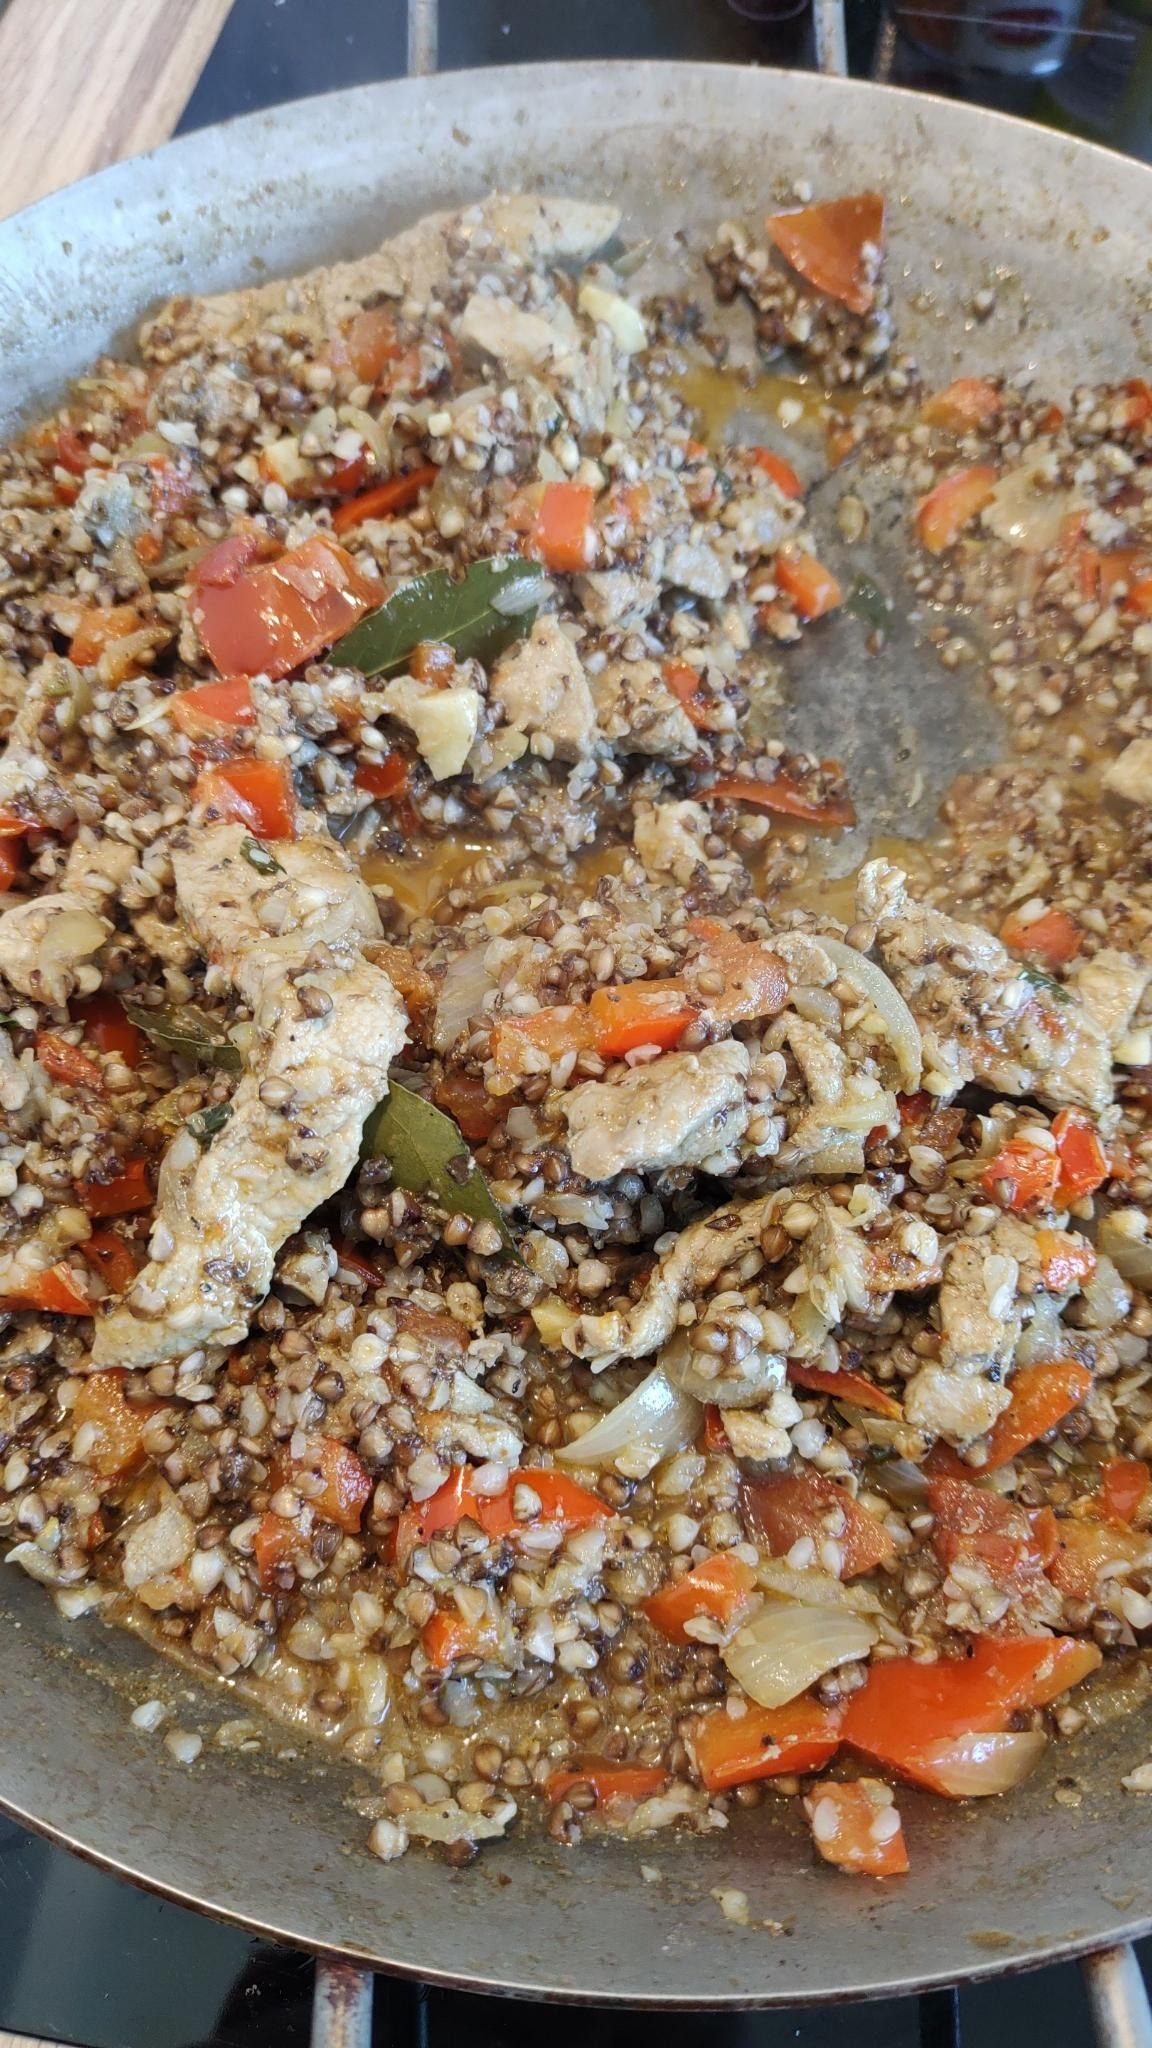
\includegraphics[angle=90, width=.5\textwidth]{lasse/Buchweizenpfanne.jpeg}
\end{figure}
\begin{recipe}
    [ % Optionale Eingaben
        preparationtime = {\unit[45]{min}},
        portion = \portion{3-4},
        %calory,
        source = Lasse
    ]
    {Leckere Pfanne}
    
    \introduction{
        \# Resteverwertstoffhof
    }
    

    \ingredients
    {% Zutatenliste
        \unit[500]{g} & Geschnetzeltes Geflügel \\
        \unit[1]{Tasse} & Buchweizen \\
        \unit[2.5]{Tassen} & Wasser \\
        1 & Paprika \\
        2 & Große Tomaten \\
        2 & Zwiebeln \\
        Wohlfühl & Knoblauch \\ 
        Gewürze & Pfeffer, Salz, Curry, Paprika
    }
    
    \preparation
    { % Schrittweise Zubereitung
        \\
        Die Zwiebeln schälen und schön klein schneiden. Die Paprika und die Tomaten waschen und in kleine Quadrate schneiden. Die gewünschte Menge Knoblauch vorbereiten.  \\
        
        Das Fleisch mit den Zwiebeln anbraten. Sobald das Fleisch durch ist die Paprika und die Tomaten mit dem Knoblauch hinzugeben, nochmal zehn minuten unter geschlossenem Deckel im eigenen Saft braten. Hier mit Curry, Salz, Pfeffer würzen und ein Lorbeerblatt hinzugeben. 
        Den Buchweizen kurz auswaschen. \\
        
        Das Wasser in die Pfanne geben und den Buchweizen unterrühren. Die Hitze der Pfanne hoch drehen, dass das Wasser schnell wieder kocht. Solange offen köcheln, bis der Buchweizen sämtliches Wasser aufgenommen hat, dabei ab und zu über den Boden rühren.         Feddich :D
        
    }
    
    \hint
        {% Hinweise
        Schmeckt sehr gut auch mit einem Löffelchen Schmand im Teller. 
        
        Zusätzlich zur Paprika bietet sich eigentlich jegliches Gemüses und Konsorten an, die gerade weg müssen. Und geht natürlich auch alles ohne Fleisch, dann tut aber ein bisschen Butter oder Margarine gut. 
        
        Das Bild wurde von einem glücklichen Koch generiert.
        }
    
    \end{recipe}
    